% $Id: tamdoc.tex 3956 2007-05-14 10:52:14Z loizides $

\documentclass{article}
\usepackage{enumerate,epsfig,geometry}
\geometry{letterpaper}
\usepackage{ifpdf}

\ifpdf
 \usepackage[pdftex,backref,pagebackref,colorlinks,
             linkcolor=blue,citecolor=blue,anchorcolor=blue,
             pagecolor=blue,urlcolor=red,a4paper]{hyperref}
 \pdfcompresslevel=9 % compression level for text and image;
 \pdfadjustspacing=1 % same spacing as latex
 \pdfcatalog{/PageMode(/UseOutlines)} % or UseNone
 \pdfinfo{
  /Title           (Tree Analysis Modules)
  /Author          ()
  /Creator         ()
  /Producer        (pdfTeX \pdftexversion\pdftexrevision)
  /CreationDate    (\today)
  /Subject         ()
  /Keywords        ()
 }
%
\else %pdffalse
%
 \usepackage[ps2pdf,backref,pagebackref,colorlinks,
             linkcolor=blue,citecolor=blue,anchorcolor=blue,
             pagecolor=blue,urlcolor=red,a4paper]{hyperref}
 \hypersetup{
   pdftitle    = {Tree Analysis Modules},
   pdfauthor   = {},
   pdfcreator  = {},
   pdfproducer = {},
   pdfsubject  = {},
   pdfkeywords = {}
 }
\fi

% not known by latex2html
%\graphicspath{ {./pics/} }

%%%%%%%%%% Start TeXmacs macros
\newenvironment{itemizedot}
  {\begin{itemize}\renewcommand{\labelitemi}{$\bullet$}\renewcommand{\labelitemii}{$\bullet$}\renewcommand{\labelitemiii}{$\bullet$}\renewcommand{\labelitemiv}{$\bullet$}}{\end{itemize}}
\newenvironment{itemizeminus}
  {\begin{itemize}\renewcommand{\labelitemi}{$-$}\renewcommand{\labelitemii}{$-$}\renewcommand{\labelitemiii}{$-$}\renewcommand{\labelitemiv}{$-$}}{\end{itemize}}
\newcommand{\tmem}[1]{{\em #1\/}}
\newcommand{\tmstrong}[1]{\textbf{#1}}
\newenvironment{enumeratenumeric}{\begin{enumerate}[1.]}{\end{enumerate}}
%%%%%%%%%% End TeXmacs macros

\begin{document}

\title{Tree Analysis Modules} 
\author{Maarten Ballintijn , Constantin Loizides and Corey Reed} 
\maketitle

{\tableofcontents}

\newpage

\section{Introduction}

\subsection{What is TAM?}

The Tree-Analysis Module (TAM) package was developed with three main goals in
mind. First, to provide a very general, modular framework for analyzing data
in ROOT trees. Second, to ensure compatibility with Proof and allow users to
switch between PROOF-based and PROOF-less analysis with as much ease as
possible. Third, to hide, as much as possible, all direct interaction with the
tree itself from the user. % Add a a few more lines

\subsection{Organization}

The TAM package depends only on a few ROOT objects. Though originally
conceived in order to process Phobos analysis trees (AnTs), TAM is based on
two general ideas from ROOT: the TSelector method for processing trees and the
TTask structure for creating and running a hierarchy of modules. Currently the
entire TAM package consists of only three classes:
\begin{itemizedot}
  \item TAModule - The base class for all user modules.
  
  \item TAMSelector - Provides the (hidden) interaction with the data loaders.
  
  \item TAMOutput - Stores output objects for all modules, preserves the
  module hierarchy and handles the merging of all modules' output objects
  under PROOF.
 \item TAMVirtualLoader -  Defines the interface for the loader plugins.
 
 \item TAMVirtualBranchLoader - Defines interface for virtual branch loaders.

 \item TAMTreeLoader - Loads tree branch loader into TAM.

 \item TAMTreeBranchLoader - Loads actual branch of the tree.

 \item TAMBranchInfo - Manages information for a branch such as the branch's name and type.

\end{itemizedot}
These classes can be found in the \$ROOTSYS/include or tam/inc directories.

\section{Getting Started With TAM}

\subsection{The Module Concept}

An analysis performed using TAM consists of a hierarchy of modules, each of
which can access any or all branches in the tree. In principal, each module is
independent of the other modules at the same level in the hierarchy; TAM
provides functionality for getting the list of submodules from any given
module, but does not provide direct access to parent or neighbor modules.
There is no restriction placed on modules inheriting from TAModule from
implementing such functionality, however.

At any level in the module hierarchy, a module has the ability to stop
processing in a variety of ways: stopping itself and its submodules from
further processing of the current execution task (i.e. the current tree entry
in Process(), or the SlaveTerminate() function), stopping all modules from
further processing of the current execution task, or stopping all modules from
any further processing. Such functionality is ideal for proper error handling
and for modules dedicated to performing event selection.

Processing of the tree is performed similarly to the TSelector methodology.
The user does not need to explicitly call any of the main execution tasks of
the modules (Begin(), Process(), etc.) as these are automatically called at
the appropriate time by the selector. User-made modules should also never need
to directly access the tree. Thus, knowing the entry number of the entry the
module is currently processing should not be necessary (indeed, it is hidden).

Typical analysis by a module would proceed as follows:
\begin{itemizedot}
  \item Make all histograms and request all branches in SlaveBegin().
  
  \item Load and process all data in Process() (i.e. fill histograms).
\end{itemizedot}
In its most simple form, this is all that is required. The TAM facility takes
care of reading the data from the tree, storing the output objects (e.g.
histograms) and making sure that they are correctly merged when the analysis
is run under PROOF.

\subsection{Making a Module}

To process data using TAM, one must first make a module. All TAM modules:
\begin{itemizedot}
  \item Must inherit (publicly) from TAModule.
  
  \item Have a member pointer for each branch of the tree they want to use.
  
  \item Overload the following functions as necessary:
  \begin{itemizeminus}
    \item Begin() to run startup code on the client computer.
    
    \item SlaveBegin() to run startup code on the computer doing the data
    analysis.
    
    \item Process() to process an entry of the tree.
    
    \item SlaveTerminate() to run finishing code on the computer which did the
    data analysis.
    
    \item Terminate() to run finishing code on the client computer.
    
    \item Notify() to perform some tasks whenever a new file is loaded by the
    selector.
  \end{itemizeminus}
  \item Use ReqBranch(branch name, pointer) in SlaveBegin() to request each
  branch the module will need to load.
  
  \item Use LoadBranch(branch name) to load the data from the tree and set
  their pointer to point to the data.
  
  \item May contain any number of submodules which will automatically execute
  (unless explicitly set to be inactive).
\end{itemizedot}

\subsection{An Example Module}

There is an example module ExampleMod with TAM that can be found in the example
directory of TAM. This class demonstrates the usage of some basic TAM functionality.
It is a simple module which reads some data from the tree Event.root generated in 
the  ROOT tutorial ``Creation of a ROOT tree''. The simple module does some event 
selection, fill/displays two histograms, and saves them in an output file.
Additionally, there is an example macro called ReadTAM.C for using the example 
module to process a Tree in event.root. %both using Proof and without using Proof
For more information, see the ReadMe.txt in the example directory.

\subsection{Getting Data From The Tree}

Under TAM, data is read from the tree branch by branch. This is done not only
for simplicity, but also to ensure efficiency. For example, in most analysis
there will be some sort of selection which will need to be performed on each
entry of the tree. In this case, one should read only those branches which
contain the data necessary to do the selection. If an entry passes the
selection criteria, then and only then should other branches be read.

\subsubsection{Reading Branches Storing Objects}

A module will need a pointer for each branch that it will want to use. The
simplest example of this is when a branch contains an object. For example,
ExampleMod will be using a superbranch from a Tree with leaves such as
fNtrack and fTemperature:
\begin{itemizedot}
  \item ``event'' is a superbranch that stores all the objects in tree ''T''.
 
\end{itemizedot}
So it has one member variables:
\begin{verbatim}
class ExampleMod : public TAModule {

private:
   // my branches 
   Event*            fEvent;      //! the event superbranch

\end{verbatim}

A pointer may have to point to an object that is from  a derived class. Although
the module may not use any members or functions specific to the derived class, the module
should still use a pointer to this class and not its base class. This is because, at least 
in principal, the derived class may contain more information, so we need to make sure the 
extra memory is allocated to allow this extra information to be read into memory correctly. 
The type checking performed by the TAMSelector each time a new tree is loaded will ensure 
that the correct type of pointer is used. {\tmstrong{NOTE:}} Since version 1.0 of TAM one 
may use also pointers to a base class: TAM will always make sure that the right pointers 
are allocated.

The class then initializes its pointers to null.
\begin{verbatim}
ExampleMod::ExampleMod(const Char_t* name, const Char_t* title) :
   TAModule(name, title),
   fEvent(0),
   fNtrack(0),
   fTemperature(0),
   fNtrackhist(0),
   fTemphist(0)
   {
   }
\end{verbatim}
{\tmstrong{NOTE:}} These pointers should {\tmem{NEVER}} be made to point to an
object created with \verb�new�! Doing so can cause a memory leak, since the
TAMSelector can change the values of these pointers once any module calls
LoadBranch(branch name).

\subsubsection{Reading Branches Storing Numbers}

If the data stored in a tree is not an object, then the user will need to
declare a class or struct whose member variables corresponds to the leaves of
the branch. Thus, for the following branch,
\begin{verbatim}
*Br 0 :MyBranch : Momentum/F:MomVec[3]/F:NumHits/I *
\end{verbatim}
A module would need to make a struct containing a Float\_t, then an array of
Float\_t's with size 3 and an Int\_t:
\begin{verbatim}
class MyNumMod : public TAModule {

public:
   struct MyBranch_t {
      Float_t fMomentum, fMomVec[3];
      Int_t fNumHits;
   };
\end{verbatim}
{\tmstrong{NOTE:}} The order, as well as the type, of the variables must match the
order of the leaves in the branch!

In order for TAM to be able to do complete type checking on such branches, any
class or struct created for reading such branches must be contained in the
TClass dictionary. This is quite a simple requirement to satisfy; simply add
the class or struct to the LinkDef file when compiling the module. For the
example above, of a nested struct, the LinkDef file would contain the
following lines:
\begin{verbatim}
#pragma link C++ class MyNumMod+;
#pragma link C++ class MyNumMod::MyBranch_t+;
\end{verbatim}
Now that a proper struct exists for the branch, the module can declare a
pointer to it in the usual way.
\begin{verbatim}
class MyNumMod : public TAModule {

public:
   struct MyBranch_t {
      Float_t fMomentum, fMomVec[3];
      Int_t fNumHits;
   };

private:
   // my branches
   MyBranch_t*    fMyBranch; //! the MyBranch branch
\end{verbatim}
{\tmstrong{NOTE:}} As in the case of reading objects, these pointers should
{\tmem{NEVER}} be made to point to an object created with \verb�new�! Doing so
can cause a memory leak, since the TAMSelector can change the values of these
pointers once any module calls LoadBranch(branch name).

It should also be noted that in the above example, all leaves of the branch
store numbers of the same size (4 bytes). In some trees, this may not be
true; there may be a branch which stores Int\_t's (4 bytes) together with
Short\_t's (2 bytes) or Double\_t's (8 bytes). In ROOT, such a branch can
not be read using a class or struct; for more information see the Root User's
Guide. When using TAM, however, a struct or class can be made, following the
above example, and the data will be read in correctly. Through complete type
checking, TAM is able to recognize this situation and read the data
appropriately. However, reading such branches will be slower
than reading branches containing objects or leaves whose types are all the
same size.

\subsubsection{Request That The Pointers Be Associated With The Branches}

Of course, declaring a pointer is not enough to allow a module to get at the
data. The next step is to associate the pointer with a branch in the tree.
This is done using the ReqBranch(branch name, pointer) function. This function
tells the TAMSelector that a module might request a branch with the given name
to be loaded during processing of the tree, and if the branch is loaded, the
module wants to use the specified pointer to access the data from the branch.

This function should only be called in SlaveBegin(). Continuing the
example:
\begin{verbatim}
void ExampleMod::SlaveBegin() {

   // request the branches i need
   ReqBranch("event",fEvent);
  
\end{verbatim}
{\tmstrong{NOTE:}} Unlike TTree::SetBranchAddress, one does not pass the address of the
pointer, but rather the pointer itself.

The ReqBranch function does not check that the pointer is of the correct type. 
This is done later by the TAMSelector whenever a new tree is loaded. The type 
checking insists that the pointer corresponds to the data stored in the branch. 
This works for both classes (that ROOT knows of) and fundamental types. 
{\tmstrong{NOTE:}} Since version 1.0 of TAM also pointers to a base class
will pass the check.

\subsubsection{Type Checking}

TAM uses type checking to be sure that the data contained in the tree
corresponds to the module's expectations. This type checking requires that
whatever pointer the module associates with a branch (via ReqBranch) be of a
type that can be found in the TClass dictionary. Type checking is performed
during Notify, thus whenever a new file is opened. TAM implements type
checking branch by branch in the following way.
\begin{enumeratenumeric}
  \item Checking if the branch stores an object, and if so, if the class of
  the object is the same as (or ---since version 1.0 of TAM--- derived from) 
  all pointers used to request the object.

  \item If the branch contains fundamental types (numbers), check if all
  pointers requesting this branch are of a known class or struct type and if
  each member of the class/struct corresponds exactly (both in order and type)
  to the leaves of the branch.
\end{enumeratenumeric}

\subsubsection{Load The Data}

Once the module has declared pointers for each branch and associated those
pointers with the branches, it is ready to load the actual data. This is done
using the LoadBranch(branch name) function. Once this function has been
called, the module can use its pointer to access the data for the current tree
entry.

This function should only be called in Process(). Continuing the
example:
\begin{verbatim}
void ExampleMod::Process() {

   // Load event superbranch
   LoadBranch("event");
  
\end{verbatim}
The TAM facility ensures that no branch will be read from disk more than once
during the processing of a tree entry.

\subsection{Event Selection}

Simple event selection can be done entry-by-entry during processing of the
tree. For most efficient event selection, a module should load only the
branches which contain the data needed to perform the event selection.
Ideally, a module would load only one branch at a time, performing part of the
selection to determine whether it is necessary to load the other branches.

Once a module determines that the current entry in the tree does not
pass the event selection, the module can call SkipEvent() to stop it and its
submodules from further processing of the entry. Thus one could make a single
module which handles all the event selection and contains all other analysis
modules (which depend on that event selection) as submodules.

While SkipEvent() will cause the module and its submodules to be made inactive
during the current execution task (i.e. during the Process() of the current
entry), it will of course not cease further processing of the function in
which it was called. Thus is it probable that a module will want to
\verb�return� from the function immediately after calling SkipEvent().

\subsection{Error Handling}

TAM provides some basic functionality for error handling. The function
SendError() is used to both print an error message and to specify a reaction
to the error. Its use is very similar to the TObject::Error and Warning
functions, but it has some simple error handling ability. The function is
declared as follows:
\begin{verbatim}
void SendError(const EModResult errLevel, const Char_t* location, const Char_t* formattedMsg, ...);
\end{verbatim}
The first parameter is a variable from the TAModule::EModResult enum:
\begin{verbatim}
 enum EModResult {

   kWarning,      //a problem requiring no action but just printing of a warning
   kAbortModule,  //a problem requiring this mod (and its submods) to stop
   kAbortEvent,   //a problem requiring the processing of this event to stop
   kStopModule,   //a problem requiring this mod (and its submods) to stop for the rest of the analysis
   kAbortAnalysis //a problem requiring the processing of the analysis to stop
};
\end{verbatim}

This parameter tells the TAM facility how to handle the error.
\begin{itemizedot}
  \item kWarning - Simply print the specified message as a Warning, but do 
  not alter processing.
  
  \item kAbortModule - Print the message as an Error and stop this
  module (and its submodules) from further processing. The module will return
  to its normal state upon the next execute call from the selector. That is,
  if called during Process(), the module will process the next event. If
  called during SlaveTerminate(), the module can be active again for the
  Terminate() call. There is no need to call SkipEvent() after this error 
  has been sent; the entry is skipped automatically.
  
  \item kAbortEvent - Print the message as an Error and stop further
  processing of all modules. The modules will return to their normal
  state upon the next execute call from the selector as described in
  kAbortModule. There is no need to call SkipEvent() after this error 
  has been sent.

  \item kStopModule - Print the message as an Error and stop this
  module (and its submodules) from further processing. The module will never 
  return to its normal state. That is, if called during Process(), the module
  will  not process any further events. There is no need to call SkipEvent() 
  after this error has been sent; the entry is skipped automatically.
  
  \item kAbortAnalysis - Print the message as a Break and stop further
  processing of all modules completely. No module will return to its
  normal state once this error has been called. There is no need to call
  SkipEvent() after this error has been sent.
\end{itemizedot}

The SendError() function does not, of course, break out from the function in
which it is called. So while it may not be necessary to call SkipEvent() after
an error message has been sent, it probably is necessary to
\verb�return� from the function after calling SendError() with an error level
of kAbortModule or higher.

An example of using SendError() can be found in the example module:
\begin{verbatim}
void ExampleMod::Process() {

   // print a warning that Process was called on this module, but
   // don't stop processing.
   SendError(kWarning,"Process", "Function called in module [%s].",
             GetName());

   LoadBranch("event");

   if ( (strcmp(GetName(),"ExampleMod")==0 ) &&
        (fCounter > 10000 ) ) {
      // if this module is named ExampleMod, don't let it (or its submodules)
      // process events higher than 10000 (using fCounter to count events) 
      SendError(kAbortModule,"Process","Skipping module [%s].", GetName());
      return;
   }
\end{verbatim}

A module may not always wish to display a warning or error message. TAM
modules can use the Get/SetVerbosity() functions to check and change the
verbosity level of the module. {\tmstrong{NOTE:}} SetVerbosity() is not 
recursive ---it does not affect the verbosity setting of submodules. 
It is entirely up to the user to decide how a module uses (or ignores) 
the verbosity setting.

Although a module can skip its own (and its submodules') processing of the
current entry or execution task without printing an error message, via
SkipEvent(), it is not possible for a module to abort the analysis or
the current execution task for all modules without printing an error message.
SendError is by design the only way for a module to accomplish this, thus
requiring the module to give an indication of what went wrong.

\subsection{Browsing And Saving Output}

In any analysis, there will be some output objects; producing some output is
indeed the whole point of performing an analysis. Under TAM, a module can
store its output objects using the AddOutput(object) function. When running
under PROOF, the output objects will be merged (from each worker computer) and
sent back to the client computer, preserving the module hierarchy.

The module hierarchy and their output objects can be browsed in the ROOT
browser, as illustrated in fig.~\ref{fig1}.

\begin{figure}[htb!f]
\begin{center}
\ifpdf
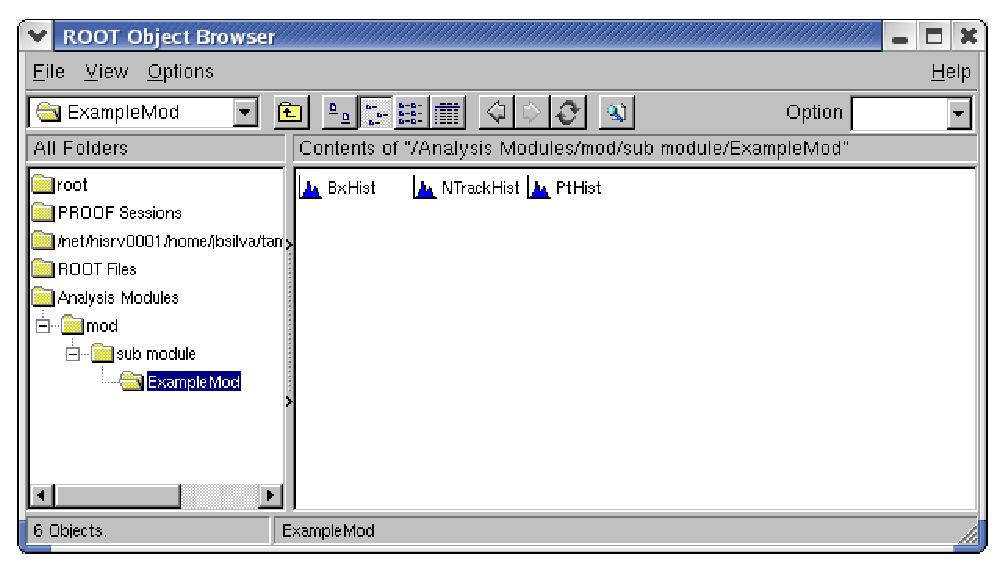
\epsfig{file=pics/outputBrowse.pdf}
\else
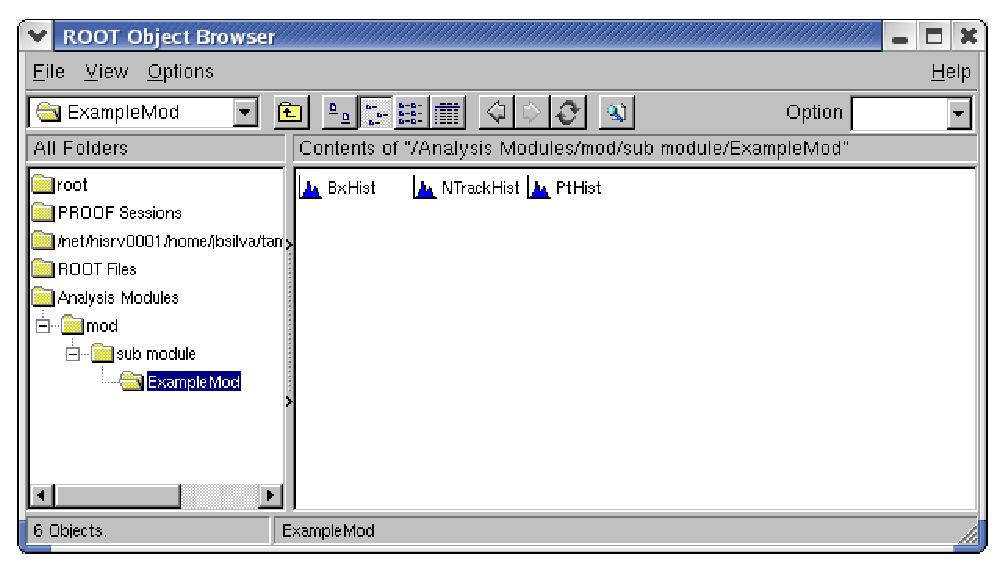
\epsfig{file=pics/outputBrowse.eps}
\fi
\caption{Root browser showing the module hierarchy 
         and their output objects}
\label{fig1}
\end{center}
\end{figure}

As an example, ExampleMod creates some histograms and adds them to its
output list.
\begin{verbatim}
void ExampleMod::MakeHist() {
   //called in SlaveBegin()
   
   fTemphist = new TH1D("T1","Temperature_Hist",40,19.5,21.5);
   AddOutput(fTemphist);
   
   fNtrackhist = new TH1D("T2","NTrackHist",50,584,616);
   AddOutput(fNtrackhist);
}
\end{verbatim}

Only objects which have added to the module's output list via
AddOutput(object) will show up in the browser. {\tmstrong{NOTE:}} when running
under PROOF, a module {\tmem{must}} call AddOuput(object) on any objects that
it wants to send back to the client computer.

The list of output objects can be saved to an output file in two ways. The
default method is to recursively go through the module hierarchy and write
each module's output objects to the file, thus flattening the hierarchy. The
other method is to explicitly save the module output object containers
(TAMOutput's), preserving the module hierarchy.

This is done by calling Write() on the output list (actually on the top-most
task's output container). This is straight forward:
\begin{verbatim}
TList* output=0;
if (runningUnderProof) {
   output = proof->GetOutput();
} else {
   output = myTAMSelector->GetModOutput();
}
// to flatten the hierarchy and dump all output objects to the file:
output->Write();
// to preserve the module hierarchy and write all output object containers
// (and output objects) to the file:
output->Write(output->GetName(), TObject::kSingleKey);
\end{verbatim}

{\tmstrong{NOTE:}} When running under PROOF, the output list may (in principal) contain
other objects besides the module output containers. If only the module output
should be written, the top-most module's output container must be extracted
from PROOF's output list:
\begin{verbatim}
TList* proofoutput = proof->GetOutput();
TList* modoutput=0;
TObject* obj=0;
TIter nextOut(proofoutput);
while ( (obj = nextOut()) ) {
   if (obj->InheritsFrom(TAMOutput::Class()) {
      modoutput = dynamic_cast<TList*>(obj);
      break;
   }
}
\end{verbatim}

The user should ensure that all module's output objects have unique names if
they are to be written to a file without the module hierarchy preserved.

If the module hierarchy is preserved when writing the output objects, the user
will need to know which objects are associated with which modules. To retrieve
an output object, the user would first get the appropriate module's output
container, via FindModOutput(moduleName), then get the output object itself
from that container, via FindOutput(outputName). An alternative is to use the
FindOutput(moduleName, outputName) function, which simply combines the two
steps. Finally, please note that the TKey functionality of ROOT provides a
way to independently of module names retrieve output objects from the file. 
You can simply loop over all TKeys in the file and look at objects that
fulfill your search criteria. For more info check the ROOT manual.


\subsection{How to transparently run with or without proof}

After you have your top TAM module (called fSuperMod) configured
the following pieces of code shows how to run without and with PROOF. 

Assuming you have a Ttree (or TChain) with the input trees called fIn,
do:
\begin{verbatim}
fSelector = new TAMSelector; 
fSelector->AddInput(fSuperMod);
fIn->Process(fSelector);
\end{verbatim}

If you have a initialized PROOF session (called fProof),
make sure you upload all packages to PROOF, especially
important to upload libTAM.tar, of course. Assuming you have
a TDSet with the input trees called fIn, do:
\begin{verbatim}
fProof->AddInput(fSuperMod);
fSet->Process("TAMSelector");
\end{verbatim}

\subsection{Output From PROOF}

TAM has been designed so that a module can be run with or without PROOF,
without requiring the user to change the module or implement special code. As
long as a module is written with the PROOF concept in mind -- that is, placing
tasks in the appropriate functions (i.e. making histograms in SlaveBegin()),
calling AddOutput(), etc.--- the module will function in the same way under
PROOF as it will when run only on the client.

Aside from properly merging output objects, one of the main issues in making
the use of PROOF transparent to the user has been recovering the output
objects themselves from the output list. To illustrate the problem, consider
an example module, which declares a pointer to a histogram:
\begin{verbatim}
class Example2Mod : public TAModule {
private:
   // my histograms
   TH1F*   fh40;     //! channel (4,0)
\end{verbatim}

Initializes the pointer to 0 everywhere the module is created (both on the
client and worker computers):

\begin{verbatim}
Example2Mod::Example2Mod(const Char_t* name, const Char_t* title) :
   TAModule(name, title),
   fh40(0),
\end{verbatim}
{\tmem{On the worker computer}}, assigns the pointer to point to a new
histogram:
\begin{verbatim}
void Example2Mod::MakeHist() {
   // called during SlaveBegin()

   fh40 = new TH1F(\"fh40\",\"(4,0)\",100,-5.0,595.0);
   AddOutput(fh40);
\end{verbatim}

Then tries to directly use this pointer to access the histogram during
Terminate() ---i.e. on the client computer:
\begin{verbatim}
void Example2Mod::Terminate() {
   fh40->Draw();
\end{verbatim}

{\tmstrong{NOTE:}} When the module is run on the client without PROOF, this 
code will work fine. However, under PROOF, the module which exists on the client
computer would never have run SlaveBegin; so the pointer would still be
null in Terminate(), causing the module to crash.

Thus the user would be forced to change the code so that it worked under PROOF
---by searching the module's output list and assigning the pointer to the
appropriate output object.

TAM does this automatically; allowing the user to create a module as shown in
the example and have it work both with and without PROOF. To facilitate this,
when running under PROOF, TAM will:
\begin{enumeratenumeric}
  \item Cache some information about all of the module's member variables.
  
  \item Whenever AddOutput() is called, on the worker computer, check
  if the argument of the output is a member variable of the module.
  
  \item If so, check that the member variable is actually a pointer to an
  object (as opposed to a pointer to a pointer or an instance of an object).
  
  \item Store information associating the member variable's name,~{\tmem{V}},
  with the output object's name,~{\tmem{O}}. This information will be sent
  back to the client computer for use by the TAMSelector during Terminate.
  
  \item On the {\tmem{client}}~computer, search the module's output list for
  the object named~{\tmem{O}}.
  
  \item Set the member variable named~{\tmem{V}} (of the module on the{\tmem{client}} 
  computer ---which should be null when running under PROOF) to point to the object 
  named~{\tmem{O}}. This is done before the module runs Terminate.
\end{enumeratenumeric}

It is important for the user to be aware of this issue, as the automatic
functionality that TAM implements to resolve this issue only works
when (a) AddOutput() is called using the module's member variable and (b) that
member variable is a pointer to the output object. TAM explicitly checks,
via TClass and TDataMember, that the type of the member variable is of the
form ClassName*.

Thus, when running under PROOF, the user may have to implement code which will
search the module's output list and associate the module's member variables
with the appropriate output objects if the module uses variables such as:
\begin{itemizedot}
  \item Instances (or references).

  For example,
  declaring \verb�TH1F fh40;� and calling \verb�AddOutput(&fh40);�
  
  \item Arrays of pointers. 

  For example,
  declaring \verb�TH1F* fChanHists[10];� and calling
  \verb�AddOutput(fChanHists[0]);�
  
  \item Copies of pointers. 

  For example,
  declaring \verb�TH1F* fh40;� but calling
  \verb�TH1F* fhcopy = fh40; AddOutput(fhcopy);�
\end{itemizedot}

In principal, a more complicated algorithm could be implemented into TAM which
would handle member variables that are arrays of pointers, however currently
this feature is not being worked on.

\subsection{Passing Objects Between Modules}

\subsubsection{Accessible Anywhere, Anytime}

While modules do not necessarily have access to their parent or neighbor
modules, they are nonetheless able to send and recieve objects to and from
other modules (or even from some code outside the module hierarchy). For
example, an analysis may want to make calibration objects available to several
modules for use in every event. TAM provides this functionality with the
PublishObj(object) and FindPublicObj(name) functions.

To make an object available to any module in the analysis, a module can use
the PublishObj(object) function. This will add the object to the TAMSelector's
list of public objects, unless the object is already in the list. There are
two restrictions on what can be published:
\begin{itemizedot}
  \item Published objects must inherit from TObject.
  
  \item Each object in the published list must have a unique name.
\end{itemizedot}

The restriction on the name is in place to ensure compatibility with Proof.
Once in the list, any module can retrieve this object.

FindPublicObj(name) can be used by any module to get an object from the
published object list. Currently it is only possible to search for an object
by name. If no object is found in the list with the specified name, a null
pointer will be returned.

Before a module \verb�delete�'s an object which it has published (or, if the
object was on the stack, before it goes out of scope), the module should
remove the object from the list of public objects to prevent dangling pointer
issues. This is done with the RetractObj(name) function. Note that again,
there is no RetractObj(object pointer) function. This is to prevent modules
from calling FindPublicObj(name) and then sending the result to RetractObj();
only one call to RetractObj(name) is required. RetractObj(name) will remove
the object from the list and return a pointer to the object. If no object with
the specified name was found, it will return a null pointer. Once an object
has been retracted, it can no longer be retrieved by other modules from the
list of published objects.

\subsubsection{Accessible Anywhere During Current Event}

It may be desirable to pass certain objects from one module to another for
processing the current event. These objects would be associated with the event
---available to any module processing the event, but unavailable (and properly
removed from memory) when the processing of the event is completed. An example
would be an object storing merged and corrected hits for a set of detectors
which could then be used by several modules, but are only useful for the
current event.

TAM provides this functionality with the AddObjThisEvt(object) and the
FindObjThisEvt(name) functions. These functions are similar to the
PublishObj(object) and FindPublicObj(name) functions. There are two
restrictions on what can be added to the event:
\begin{itemizedot}
  \item Published objects must inherit from TObject.
  
  \item Each object in the published list must have a unique name.
\end{itemizedot}

The restriction on the name is in place to allow quick lookup via THashTable
using the object's name. Thus retrieving objects from the event should be
efficient.

The most important feature of adding objects to the event is that
objects added to the event will be automatically deleted when all modules have
finished processing the event. Thus, the reccomended usage is for modules to
simply leave objects in the event and let TAM take care of clearing the
memory. It is, however, possible to remove objects from the event using the
RemoveObjThisEvt(name) function. It is up to the user to delete the object
once it has been removed from the event.

\section{Extending TAM Via Data Loader Plugins}

{\tmstrong{NOTE:}} The features explained in this chapter apply to TAM versions 
1.0 and higher only.

\subsection{Data Loader Plugins}
The extension of TAM by data loader plugins allows TAM to do tasks such as 
event mixing or the converting of branches. TAM works in tandem with data
loader plugins to create virtual branches on the fly from the branches of
a single or multiple trees. On a given name of a branch TAM will first
loop over a list of given plugins to find a plugin which provides the 
(virtual) branch name. If the branch name is not provided it will browse 
the branches of the connected trees if there is any. The virtual branches 
act collectively as a single tree for analysis. Virtual branches like 
actual branches are requested and loaded by TAM modules via ReqBranch and 
LoadBranch.

\begin{figure}[htb!f]
\begin{center}
\centerline{\ifpdf
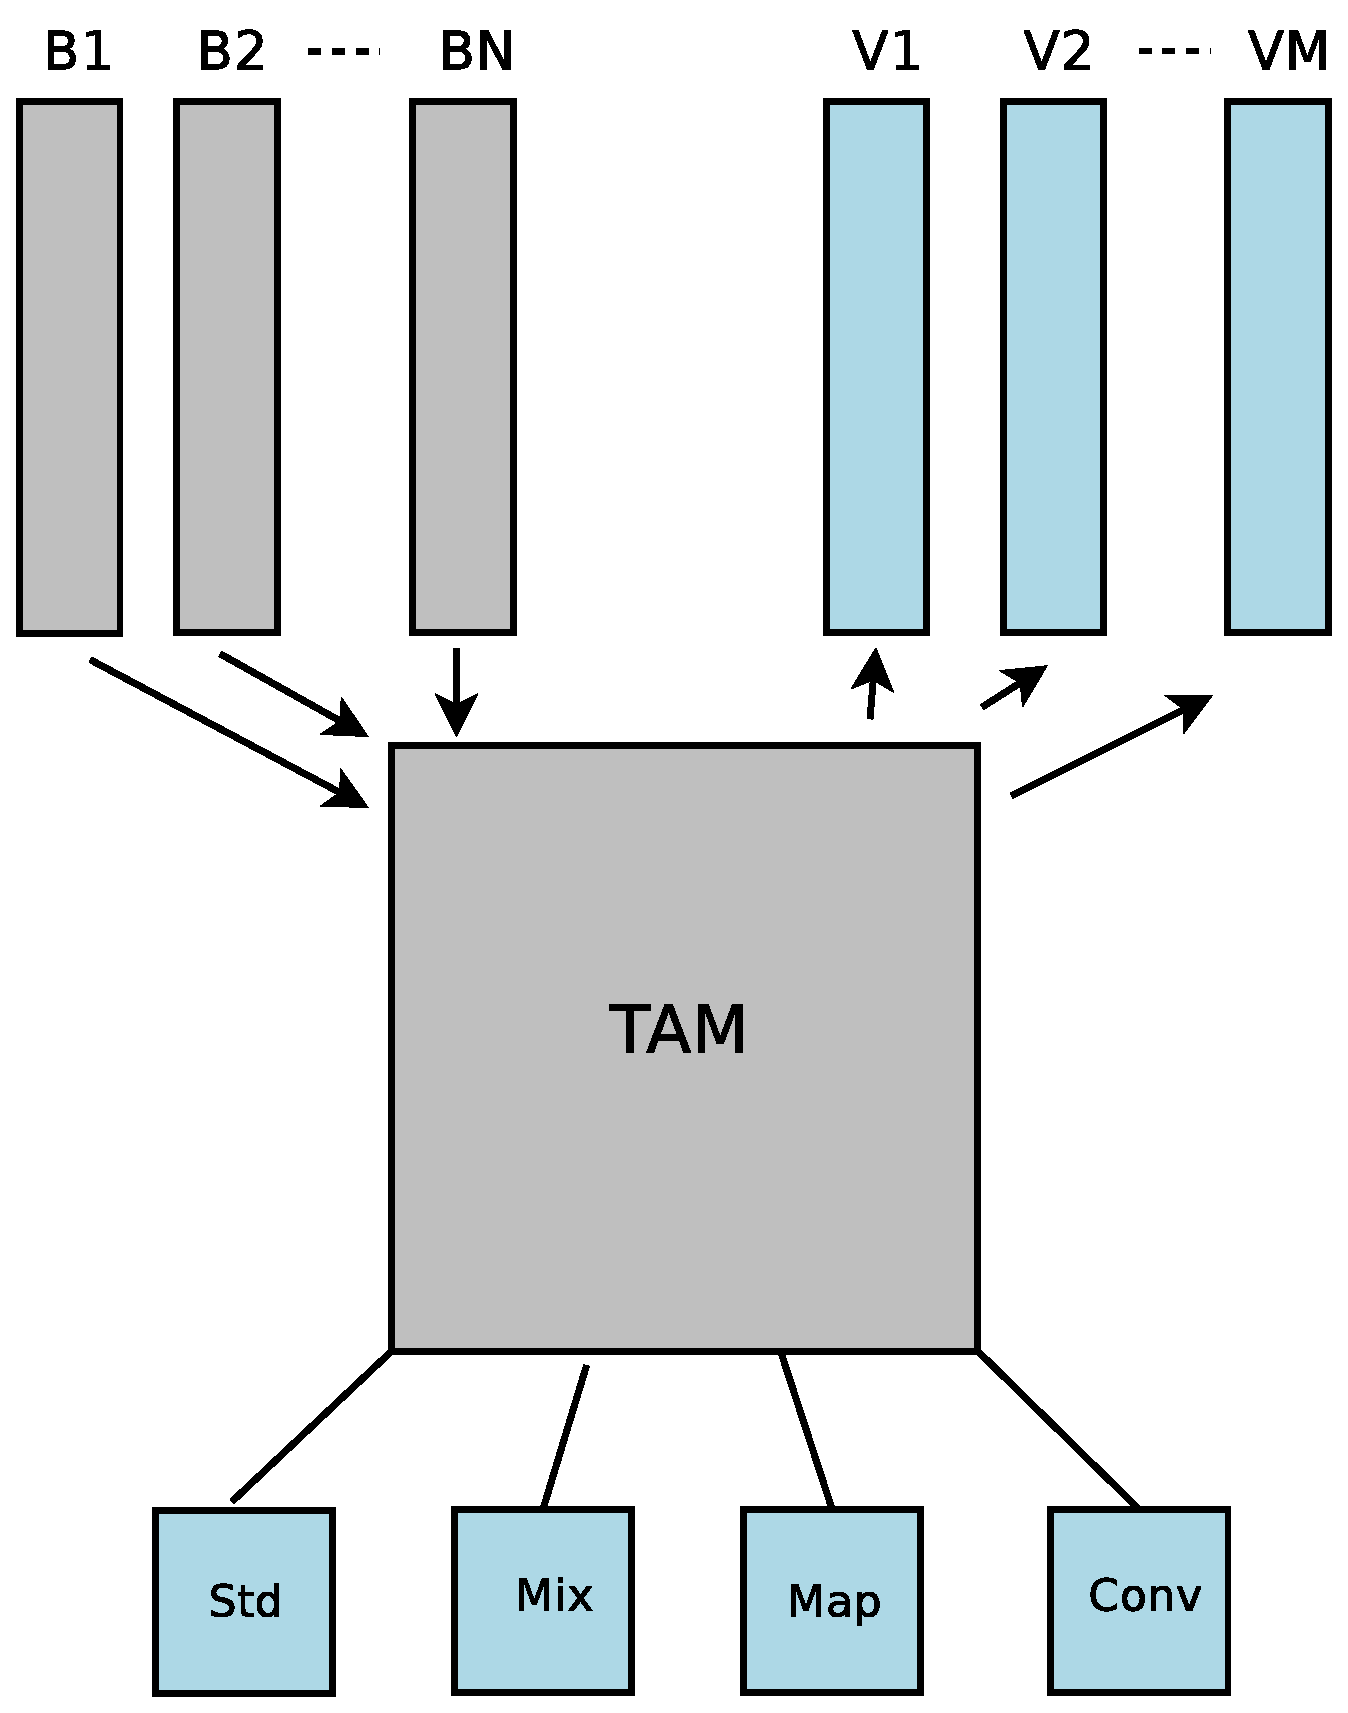
\epsfig{file=pics/virtual_branches.pdf, width=3.0in, height=2.5in}
\else
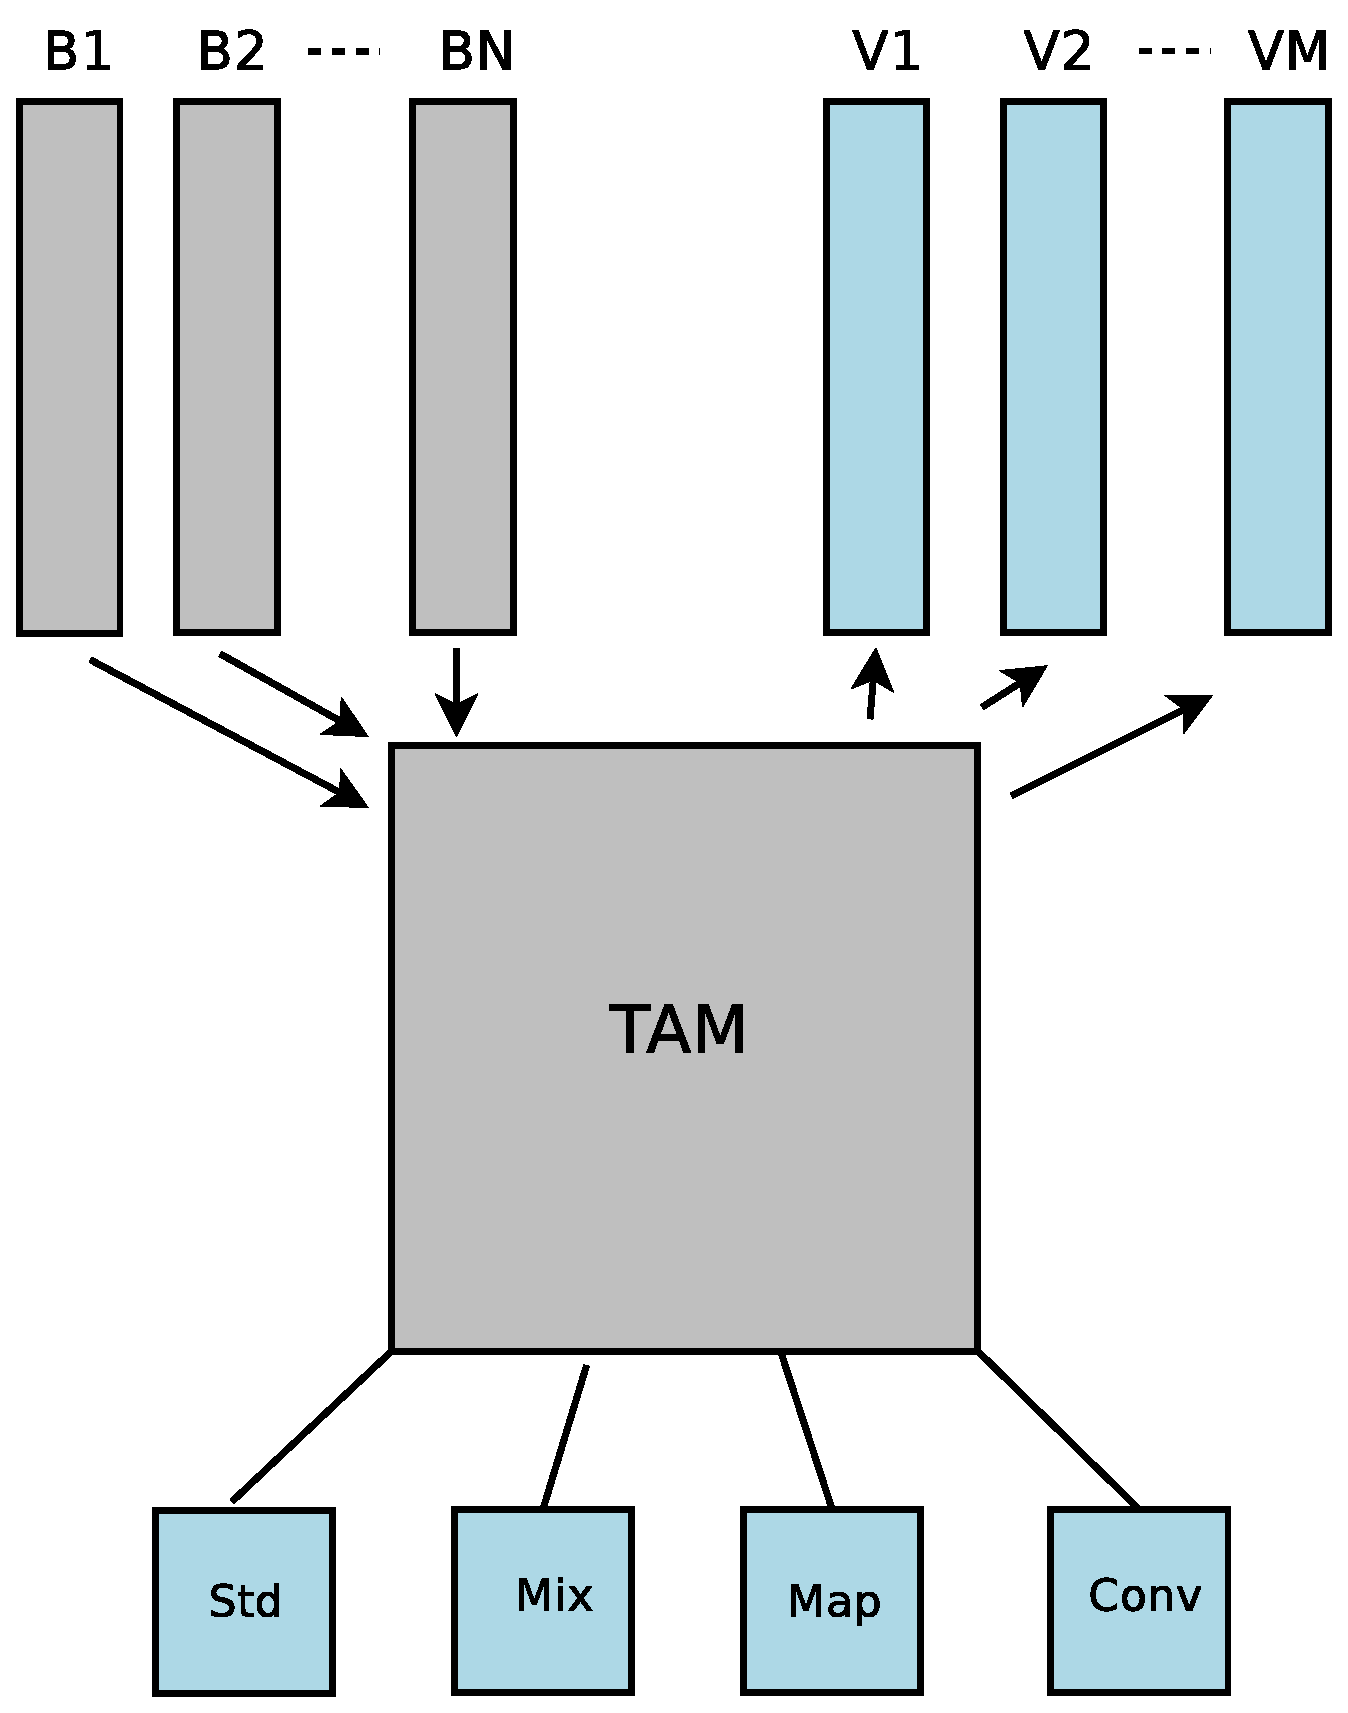
\epsfig{file=pics/virtual_branches.eps, width=3.0in, height=2.5in}
\fi}
\caption{Figure showing interface between TAM, plugins, and branches.}
\label{fig2}
\end{center}
\end{figure}

The virtual branches in TAM are never directly accessed by plugins instead
TAM serves as the interface between the two. Fig.~\ref{fig2} depicts the 
situation of TAM with various plugins and N actual branches and M virtual 
branches. The amount of virtual and actual branches are not required to be equal.
For example, consider the mixing of two identical trees where the amount of 
virtual branches equals half the amount of actual branches. However, on the 
level of the TAM modules, there is no distinction between virtual and actual 
branches.
 
For example, the plugins shown in fig.~\ref{fig2} could do the following tasks 
without the need to change any of the analysis modules. 
\begin{itemizedot}
  \item Tree Loader Plugin (Std) -  does the normal task of reading actual 
branches.
  \item Mixer Plugin (Mix) - does tree mixing and then returns the mixed 
branch to TAM.
  \item Mapping Plugin (Map) - does remapping of a branch on the fly and returns 
the remapped branch to TAM.
  \item Conversion Plugin (Conv) - does converting of  braches to be return to 
TAM for analysis.
\end{itemizedot}

\subsection{Guidelines For Writing and Loading Plugins}
This section describes how to write and load a plugin into the TAM facility.
To write your own plugin, a loader plugin must have a branch loader derived 
TAMVirtualBranchLoader and a loader derived from TAMVirtualLoader. The branch 
loader will be created by the loader. For example in the example plugin, a 
mixer loader could be declared using: 
\begin{verbatim}
class MixerLoader : public TAMVirtualLoader {
public:
   MixerLoader();
   ~MixerLoader();
   
   TAMVirtualBranchLoader*  CreateBranchLoader(TTree *tree, TAMBranchInfo* brInfo);
\end{verbatim}

All loaders are required to have a CreateBranchLoader() member function. The 
CreateBranchLoader function creates,initializes, and returns a TAMVirtualBranchLoader 
derived class object (in this example MixerBranchLoader). In the example,the branch 
loader could be declared using:
\begin{verbatim}
class MixerBranchLoader : public TAMVirtualBranchLoader {
 public:
   MixerBranchLoader();
   MixerBranchLoader(TAMBranchInfo *binfo, MixerLoader *l, TreeMixer *fTmix);
   ~MixerBranchLoader();
   
   void                   Clear(Option_t *option="");
   void*                  GetAddress() const;
   Int_t                  GetEntry(Long64_t entry); 
   Bool_t                 Notify(TTree *tree);
\end{verbatim}

All shown functions in MixerBranchLoader are required for any branch loaders. The tasks 
performed by the functions should be:
\begin{itemizedot} 
\item Clear() - Clear up data structures used by the plugin (in this example the mixer plugin).
\item Notify() - Notifies when a new file has been opened.  
\item GetAddress() - Returns the address to which pointer passed in ReqBranch() will be set to. 
\item GetEntry() - Return data for the given entry.
\end{itemizedot} 

The loader plugin must be loaded into TAMSelector using AddLoader(). For example,
the loader plugin named MixerLoader is loaded into a TAMSelector object pointer using:
\begin{verbatim}
   MixerLoader *mloader = new MixerLoader;
   Selector->AddLoader(mloader);
\end{verbatim}

\subsection{Event Mixing Example}
The documentation provides a mixing example for ROOT trees. The tam/example directory 
includes a mixing plugin for event mixing and a macro to run the mixing plugin. The example 
uses trees created in the ROOT tutorial at http://root.cern.ch/root/html/examples/MainEvent.cxx.html. 
The included rootlogon.C will; create the neccessary files, compile, and link all the mixing 
modules. The ROOT files can also be manually created in \$ROOTSYS/test using:
\begin{verbatim}
make Event
./Event  
\end{verbatim}

The command ./Event also supports arguments for number of events, split and compression 
level. The ROOT tutorial file MainEvent.cxx provides more information on the use
./Event.  
Once the ROOT files have been created and are placed in the same directory as runExampleMod.C 
the example macros can be executed. To execute the macro given the files Event1.root and 
Event2.root exist, begin ROOT in the same directory as the example macro and use:
\begin{verbatim}
.x runExampleMod.C+("Event1.root","Event2.root") 
\end{verbatim}

The output will then be saved as example\_output.root in the current directory and can
be browsed using the TBrowser.

The included files for the example and their descriptions are:
\begin{itemizedot}
\item runExampleMod.C            - Macro that can executed to run the example module on a single
                                   file or two input files. 
\item ExampleMod.[h/cxx]         - Example module header and class implementation files. Class 
                                   inheriting from TAModule that makes and fills histograms.
\item TreeMixer.[h/cxx]          - Header and class implementation files. Does actual mixing of trees and returns
                                   the mixed data. It contains an internal TreeDataLoader class that loads actual 
                                   data from tree and returns it to the Tree Mixer.
\item MixerBranchLoader.[h/cxx]  - Header and class implementation files. Loads mixed Branch.
\item MixerLoader.[h/cxx]        - Header and class implementation files.Creates Mixer Branch Loader.  
\end{itemizedot}

The macro runExampleMod.C can run the example module with an input of either 
a single ROOT tree or a two ROOT trees(in principle more trees are possible).
If the input is a single tree the macro processes and output the file. For multiple 
input files, the mixer plugin is given to the TAMSelector. The input files are 
used in a TChain that TAMSelector will process. To properly prepare trees for event
mixing and support the use of PROOF, trees are added as friends of the first tree in
the chain using AddFriend() as:
\begin{verbatim}
   chain->AddFriend(friendchain,"treealias");   
\end{verbatim}

If the mixer has been loaded and all trees to be analyzed are friends of a chain 
TAMSelector can then begin to process events. The included mixer plugin only does the 
mixing of the number of tracks and the tracks in the input files. After processing 
the events the macro writes the output file example\_output.root in the current directory. 
 
\end{document}
